\section{Collective Oscillations}

\subsection{Neutrino Self-interactions}

\begin{frame}{Neutrino Self-interactions}


\begin{columns}[T]
   \begin{column}{0.5\textwidth}

      Interaction Hamiltonian $\mathbf H_{\nu\nu}$

      \begin{equation*}
         \sqrt{2}G_{\mathrm F} n(\boldsymbol{v}') (1- \hat{\boldsymbol{v}} \cdot \hat{\boldsymbol{v}}') \rho( \boldsymbol{v}' )
      \end{equation*}

      In Flavor Isospin space
      \begin{equation*}
         -2\sqrt{2}G_{\mathrm F} n(\boldsymbol{v}') (1- \hat{ \boldsymbol{v} } \cdot \hat{\boldsymbol{v} }')  \vec s ( \boldsymbol{v}' )
      \end{equation*}

      % \only<2>{
         % \begin{tcolorbox}
            % \begin{figure}
            %    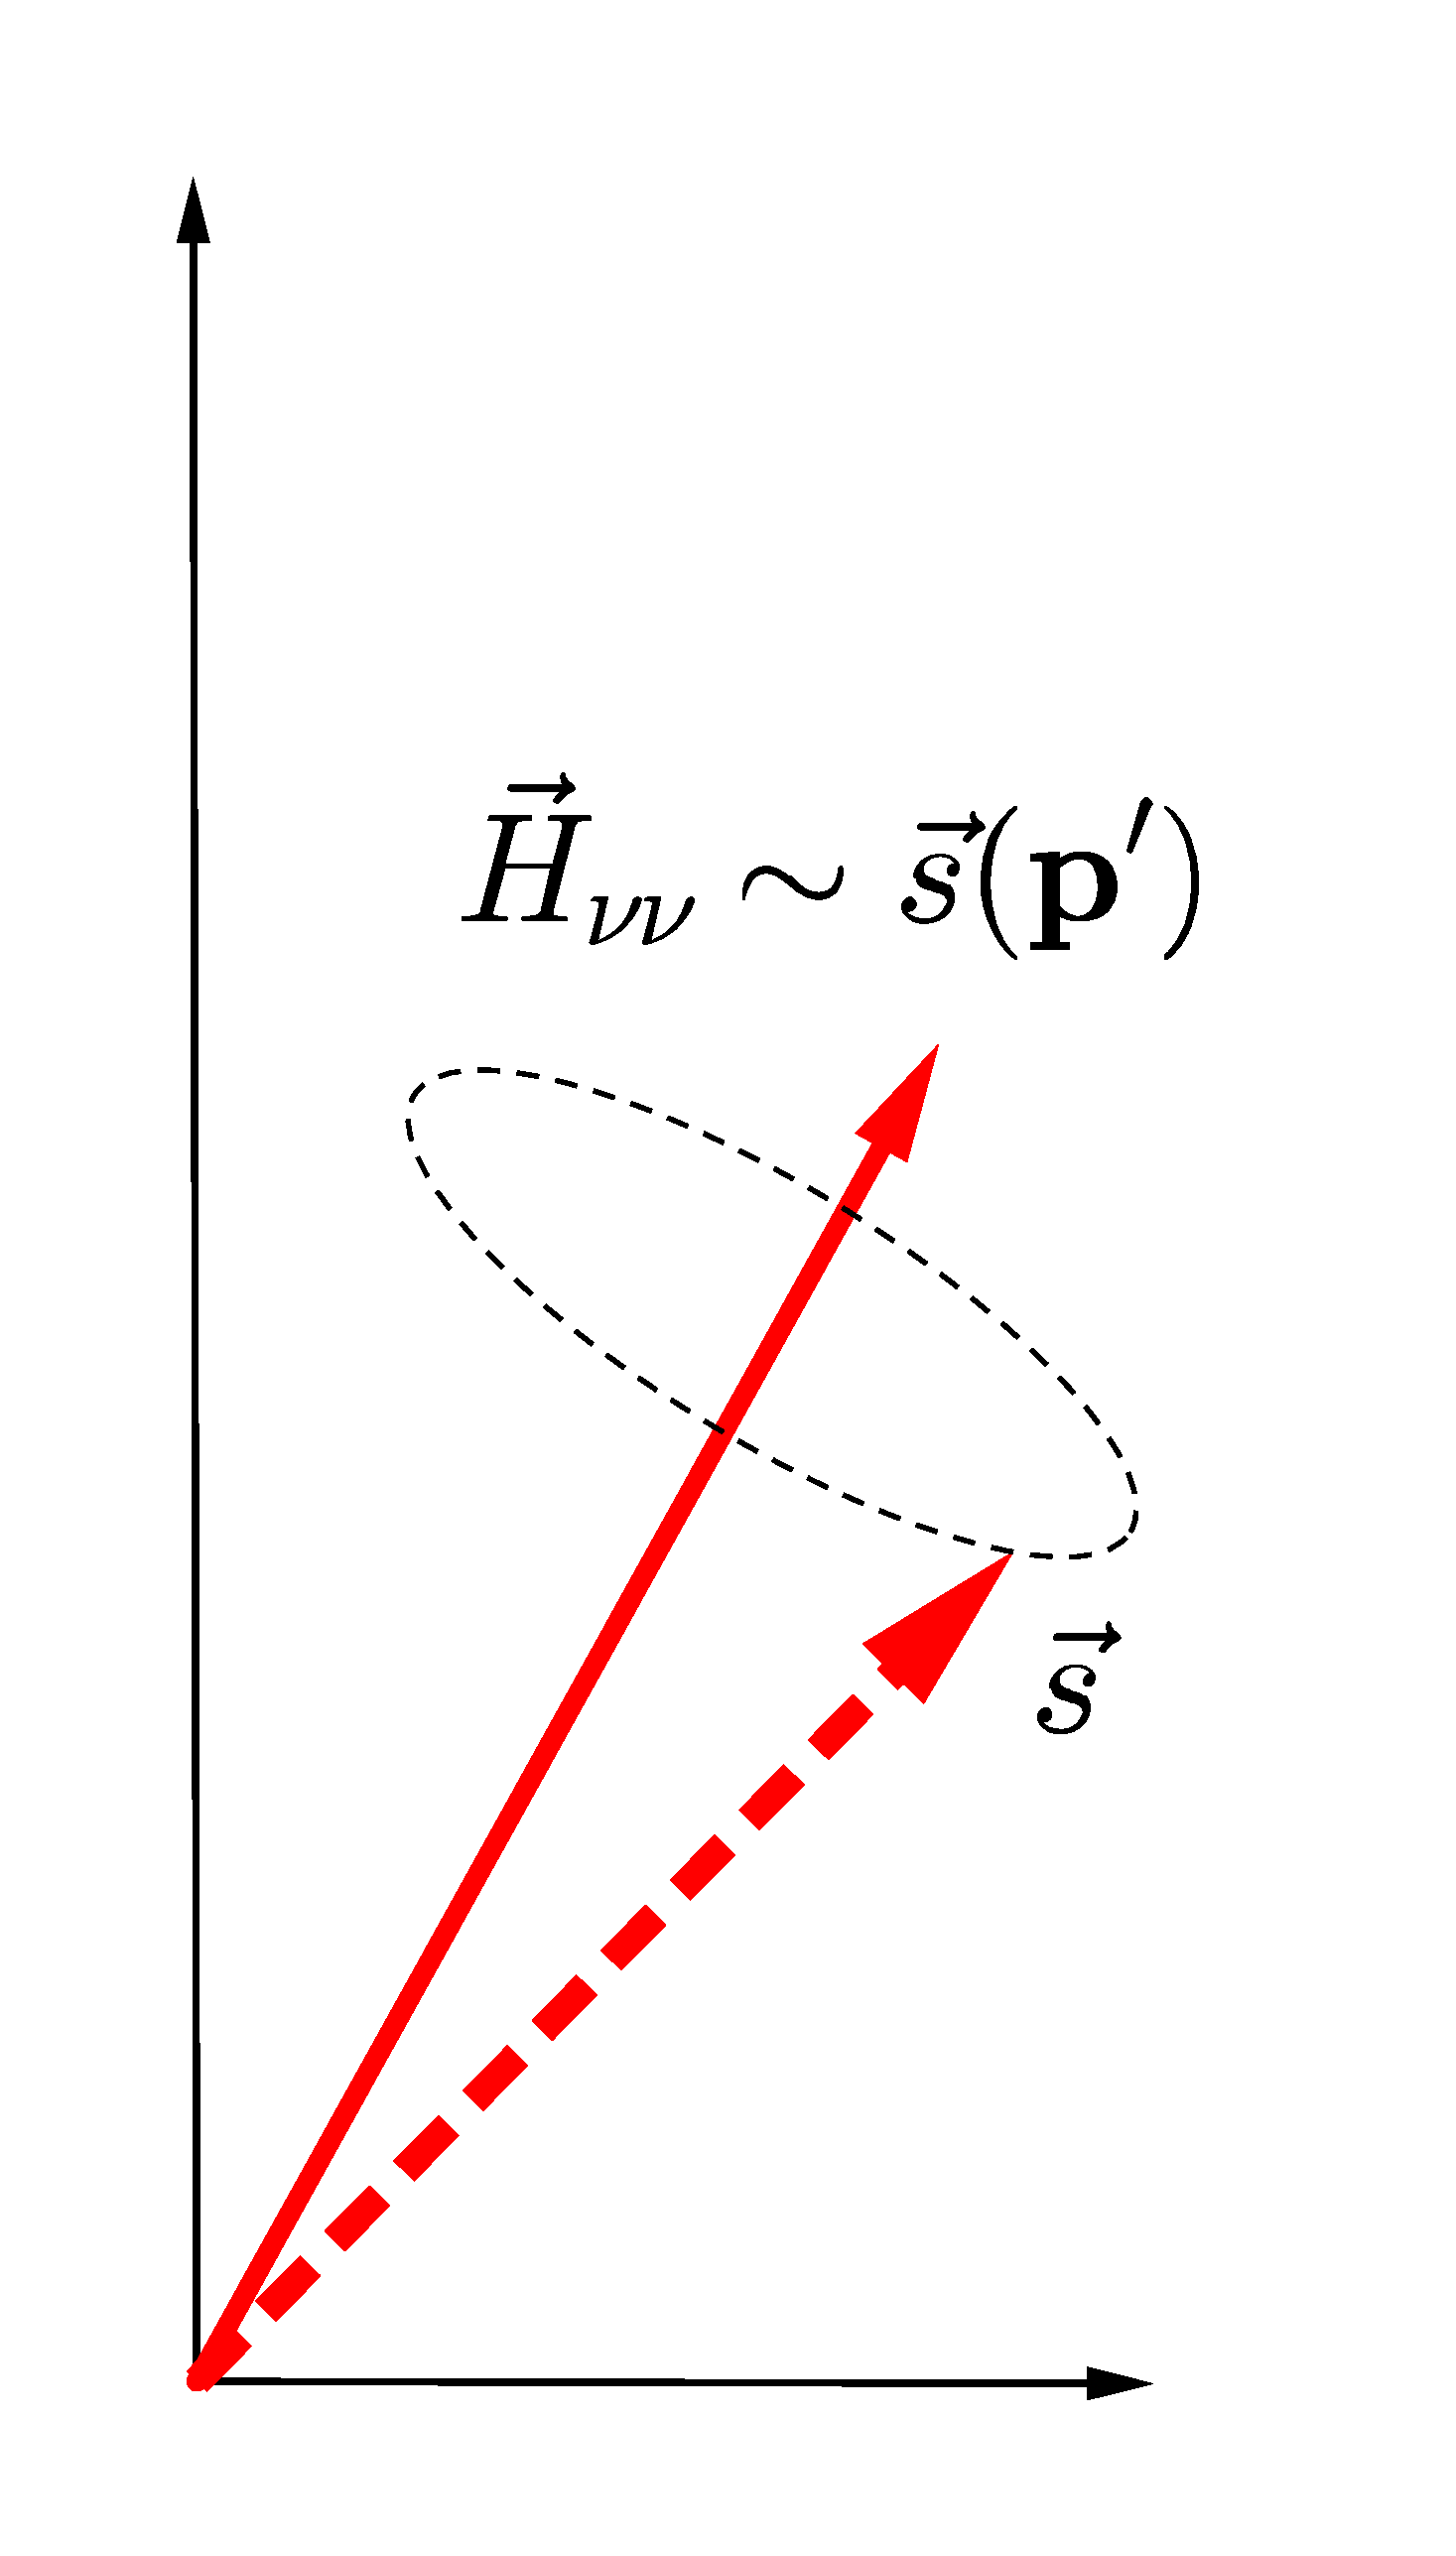
\includegraphics[width=\textwidth]{assets/self-interaction}
            % \end{figure}

         % \end{tcolorbox}
      % }


   \end{column}

   \begin{column}{0.5\textwidth}

      \begin{figure}
         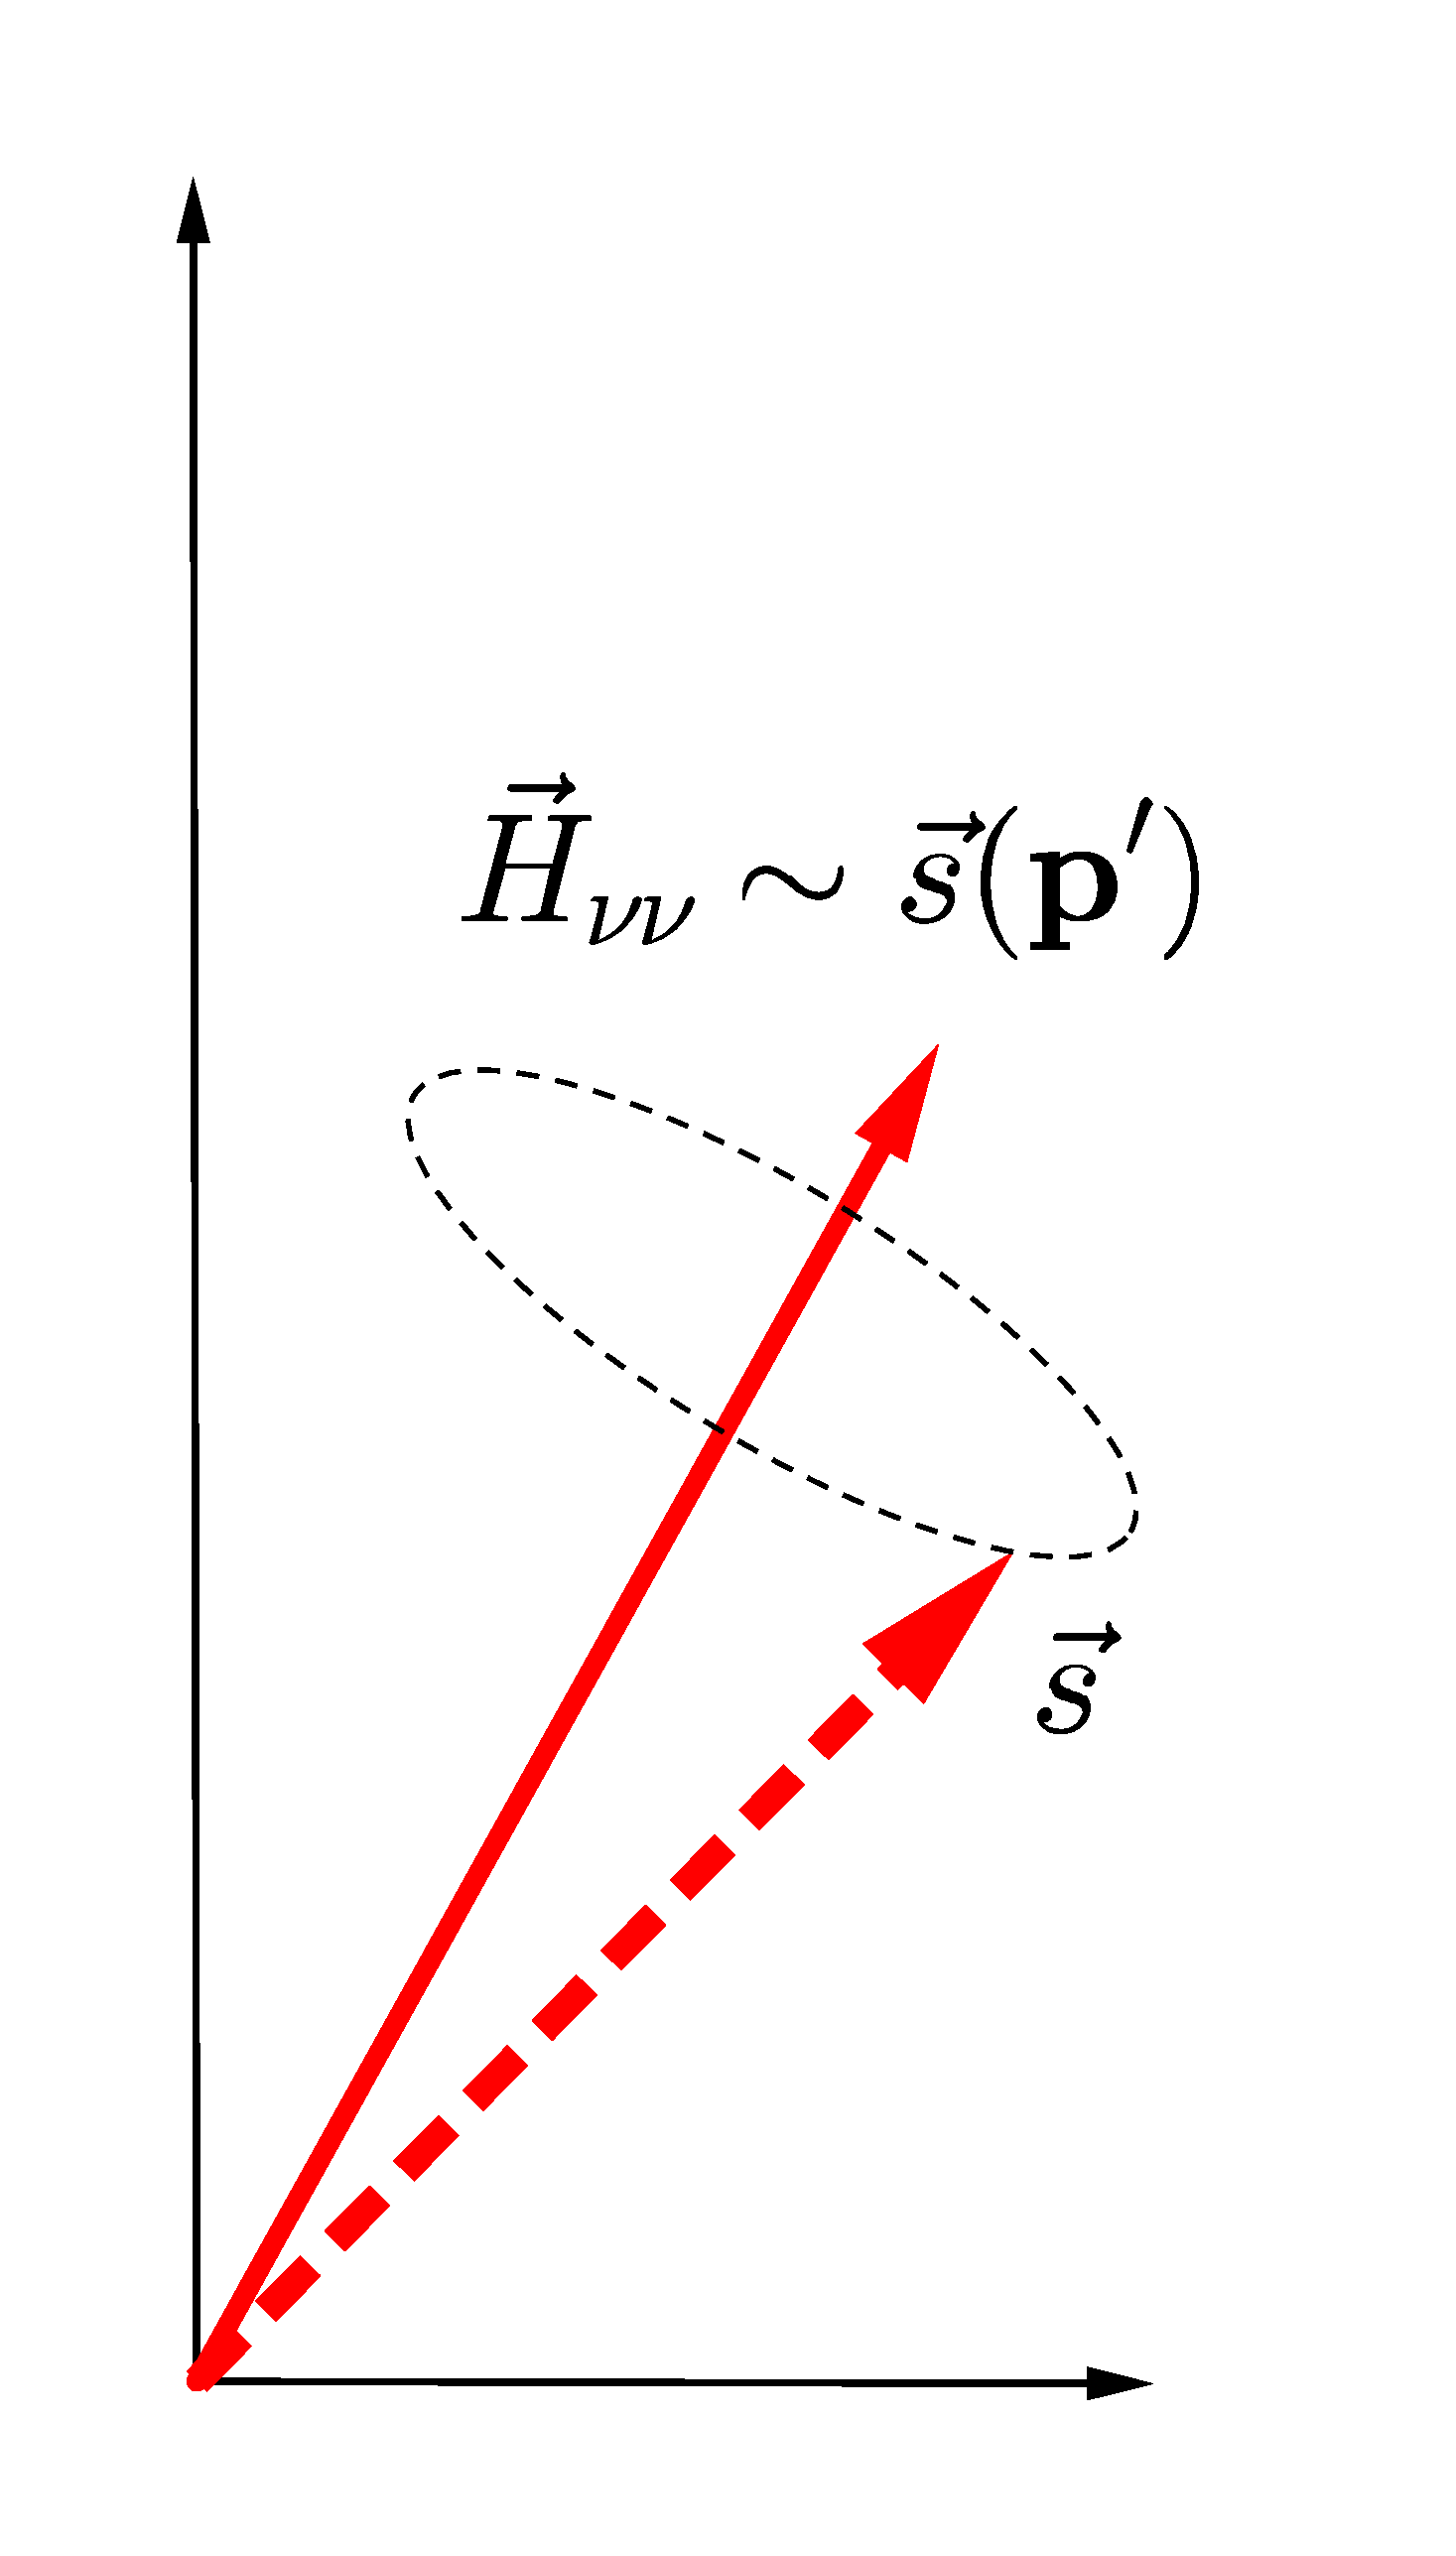
\includegraphics[width=0.8\textwidth]{assets/self-interaction}
      \end{figure}




   \end{column}


\end{columns}





\end{frame}


\begin{frame}{Neutrino Self-interactions}


   \begin{tcolorbox}[title=Characteristic Energy Scales,standard jigsaw,
    opacityback=0]

      \begin{itemize}
         \item  $\omega_{\mathrm v} = \delta m^2\big/2E $
         % \item  $\lambda \sim G_{\mathrm F} n_{\mathrm e}$
         \item  $\mu \sim G_{\mathrm F} (1- \hat{\boldsymbol{ v} }_1 \cdot \hat{\boldsymbol{v}}_2) n_{\nu} $
      \end{itemize}

   \end{tcolorbox}


\only<1>{


Vacuum oscillation oscillation frequencies
   \begin{align*}
      \omega_{\mathrm v} = \frac{\Delta m^2}{2E}  \sim& \frac{2\pi}{ 1  \mathrm{km} }  \left(\frac{\Delta m^2_{32}}{2.5\times 10^{-3} \mathrm{eV}^2 } \right) \left( \frac{1MeV}{E} \right) \\
   \sim & \frac{2\pi}{ 33  \mathrm{km} } \left( \frac{\Delta m_{12}^2}{7.5\times 10^{-5}\mathrm{eV}^2} \right) \left( \frac{1\mathrm{MeV}}{E} \right)
   \end{align*}
}

% \only<2>{
% \begin{tcolorbox}
%    \centering
%    Neutrino self-interactions might lead to faster oscillations, since $\mu \gg \omega_{\mathrm v}$.
% \end{tcolorbox}
% }

\only<2>{

Suppose we have neutrino flux $10^{50}\mathrm{ergs\cdot s^{-1}}$. We estimate the potential at radius $R$ to be

\begin{equation*}
   \mu \sim  \frac{1}{0.01 km} \left(\frac{100\mathrm{km}}{R}\right)^2 \left(\frac{1\mathrm{MeV}}{E}\right)
\end{equation*}


}


\end{frame}




\begin{frame}{Two-Beam Model}

\begin{columns}[T]

\begin{column}{0.3\textwidth}

% \begin{tcolorbox}[coltext=white,standard jigsaw,opacityback=0]
$H_{\mathrm v,1} = - \frac{1}{2}\omega_{\mathrm v} \sigma_3 $\\
$H_{\mathrm v,2} =  \frac{1}{2}\omega_{\mathrm v} \sigma_3 $\\
   % \item $H_m = \frac{1}{2}\lambda \sigma_3$
$H_{\nu\nu} = \frac{1}{2} (\mu\rho_1- \mu\rho_2)$
   % \item $H_{\nu\nu} = -\frac{1}{2}\mu_2 \rho_2$
% \end{tcolorbox}


where
\begin{equation*}
   \mu = \sqrt{2} G_{\mathrm F} \xi n
\end{equation*}

Geometric factor
\begin{align*}
\xi =& (1-\cos(\theta_1-\theta_2)) \\
=& 3/2%, \quad \text{since $\theta_1-\theta_2=\pi/2$}
\end{align*}



\end{column}

\begin{column}{0.7\textwidth}
\begin{figure}
   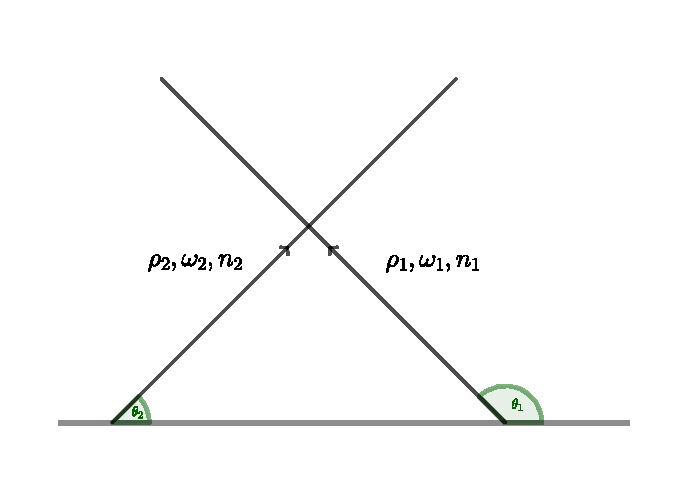
\includegraphics[width=\textwidth]{assets/two-beams-model-sym}
   \caption*{$\rho_1$: neutrinos; $\rho_2$: antineutrinos
   $\theta_1= 5\pi/6$; $\theta_2 = \pi/6$}
   $\theta_{\mathrm v}=0$
\end{figure}

% \begin{tcolorbox}[standard jigsaw, opacityback=0,coltext=white, halign=center]
%
% \end{tcolorbox}

\end{column}


\end{columns}


\end{frame}


% \begin{frame}{Two-Beam Model}
%
%    \begin{textblock*}{100pt}(220pt,10pt)
%    % \textblockcolour{black}
%    % \TPoptions{standard jigsaw, opacityback=0, coltext=white }
%    \small
%    \begin{align*}
%       H_{\nu\nu,1} = \frac{1}{2}\mu_1 \rho_1 \xi , \qquad
%       H_{\nu\nu,2} = \frac{1}{2}\mu_2 \rho_2 \xi
%    \end{align*}
%    \end{textblock*}
%
%
% \begin{columns}[T]
%    \begin{column}{0.55\textwidth}
%    \begin{figure}
%       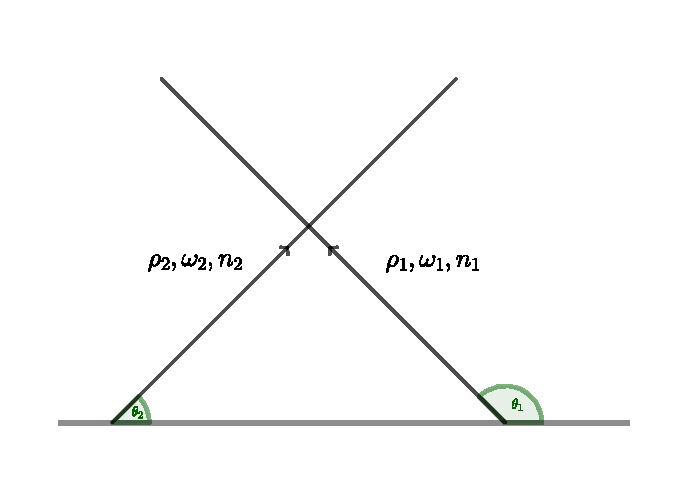
\includegraphics[width=\textwidth]{assets/two-beams-model-sym}
%       \caption*{$\rho_1$: neutrinos; $\rho_2$: antineutrinos}
%    \end{figure}
%    \end{column}%
% \begin{column}{0.45\textwidth}
%
%    \begin{equation*}
%    i \partial_z \rho_i = \left[ H_i, \rho_i \right]
%    \end{equation*}
%
%    \begin{equation*}
%    \theta_1 =  2\pi/3, \theta_2 = \pi/6
%    \end{equation*}
%
%
%
% \end{column}%
% \end{columns}
%
%
%
% \end{frame}


\begin{frame}{Neutrino Self-interactions}

\begin{textblock*}{100pt}(250pt,10pt)
Inverted hierarchy;
$\mu = 5\lvert\omega_{\mathrm v}\rvert$
\end{textblock*}

% \begin{tcolorbox}
   \only<1>{
   \begin{figure}
      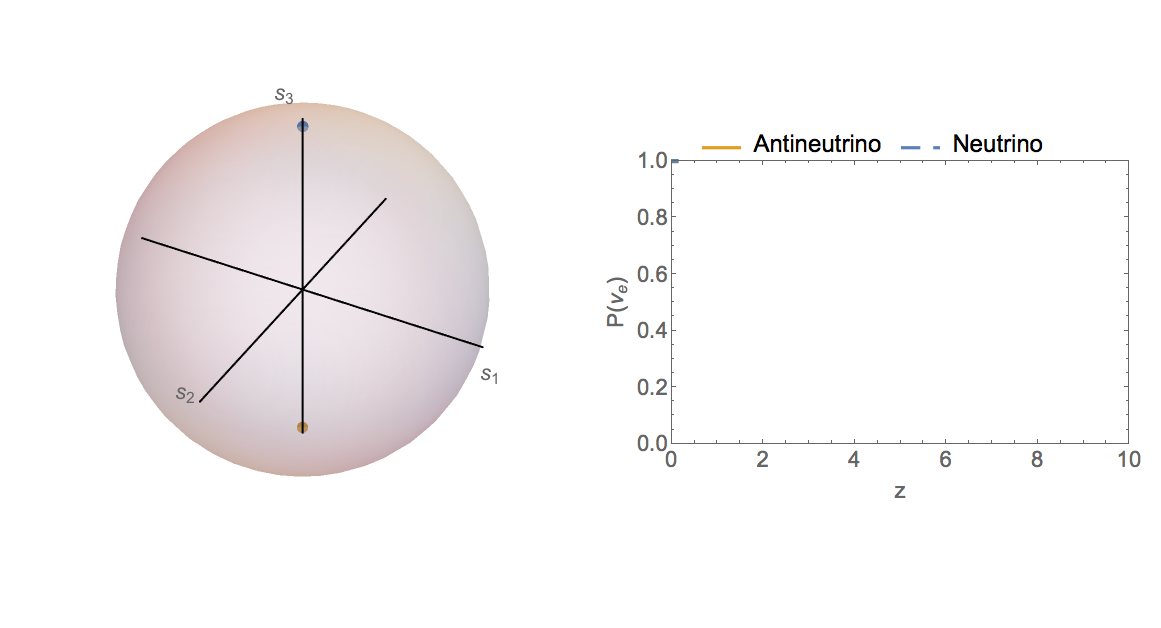
\includegraphics[width=\textwidth]{assets/bipolar-animation/bipolar-animie001.png}
   \end{figure}
   }
   \only<2>{
   \begin{figure}
      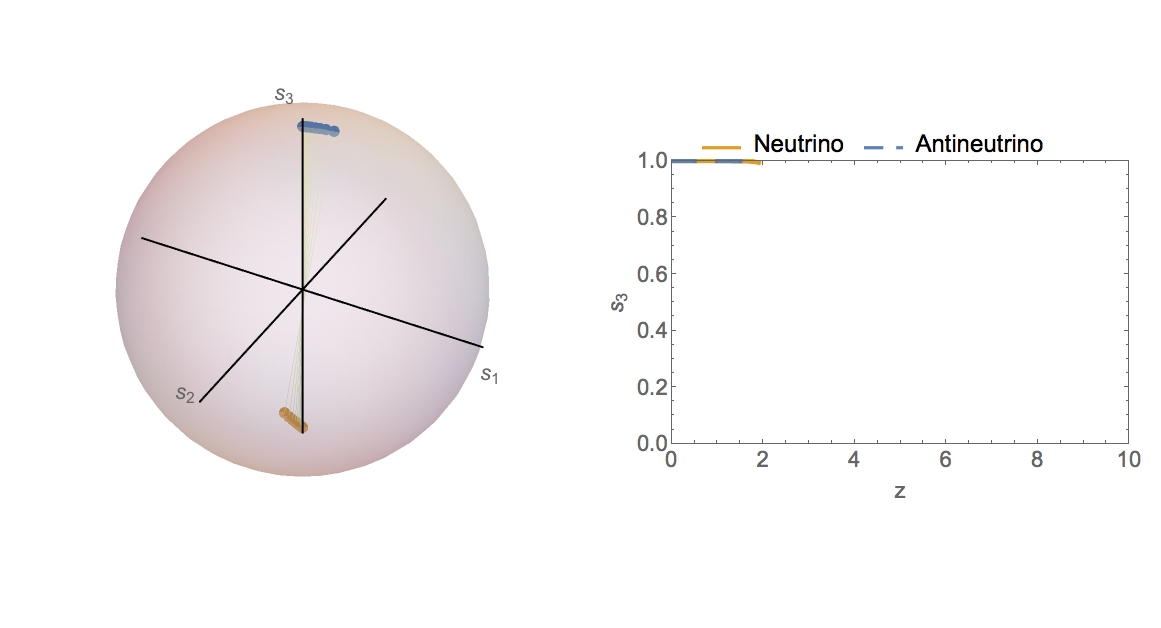
\includegraphics[width=\textwidth]{assets/bipolar-animation/bipolar-animie019.png}
   \end{figure}
   }
   \only<3>{
   \begin{figure}
      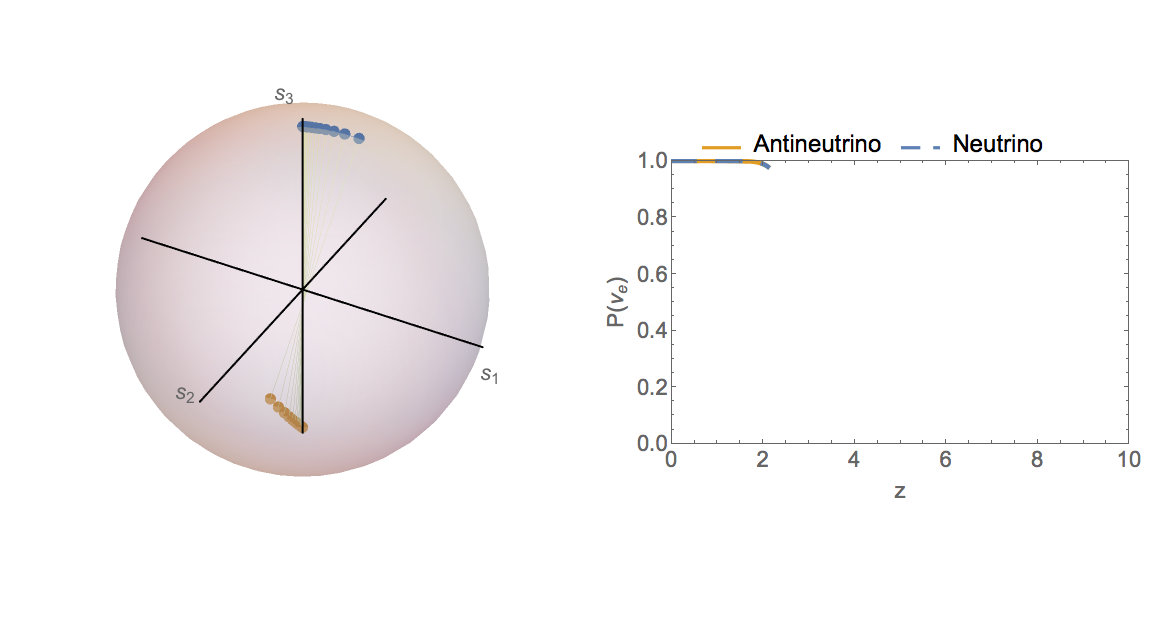
\includegraphics[width=\textwidth]{assets/bipolar-animation/bipolar-animie021.png}
   \end{figure}
   }
   \only<4>{
   \begin{figure}
      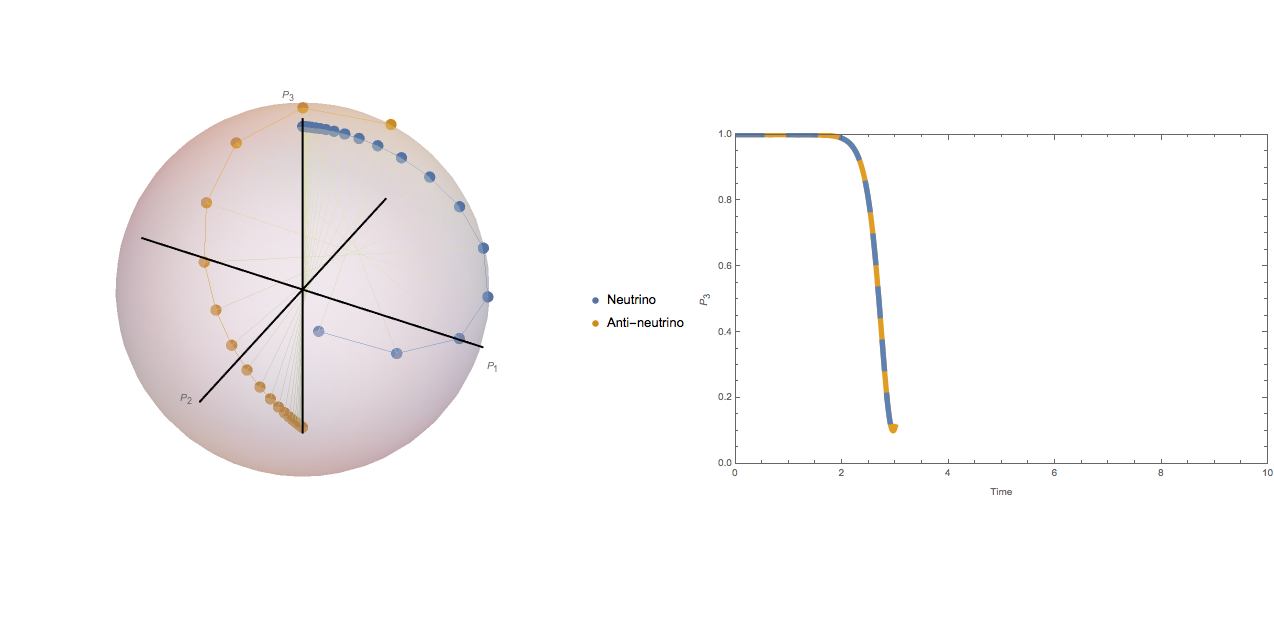
\includegraphics[width=\textwidth]{assets/bipolar-animation/bipolar-animie030.png}
   \end{figure}
   }
   \only<5>{
   \begin{figure}
      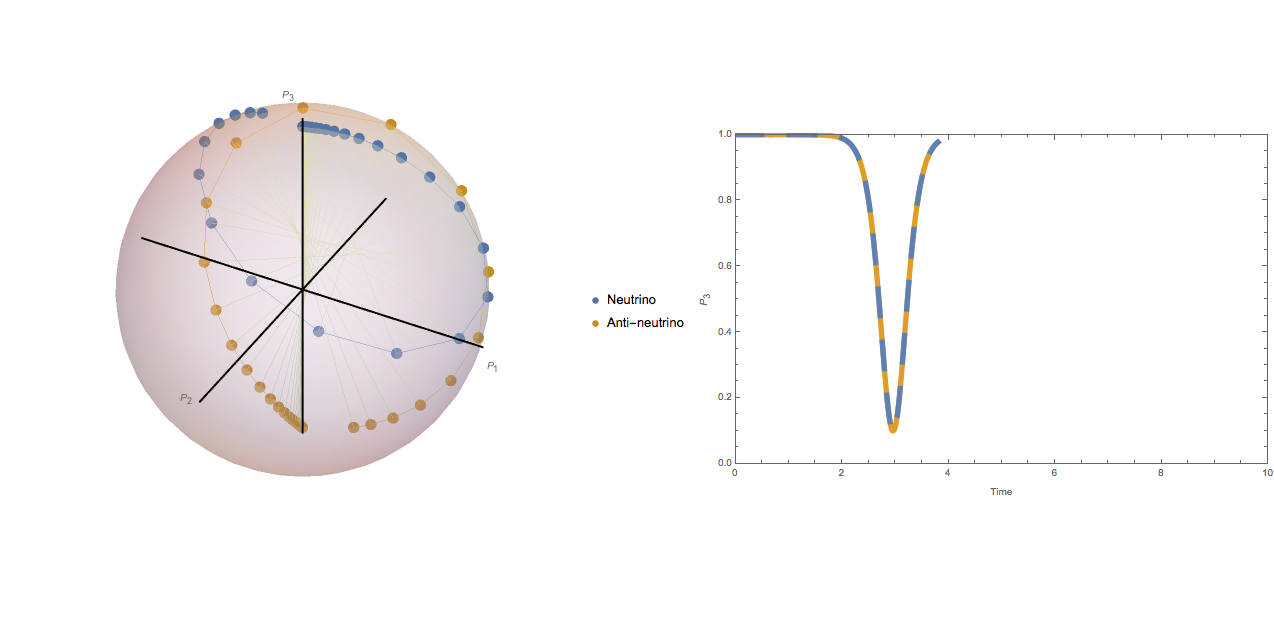
\includegraphics[width=\textwidth]{assets/bipolar-animation/bipolar-animie038.png}
   \end{figure}
   }
   \only<6>{
   \begin{figure}
      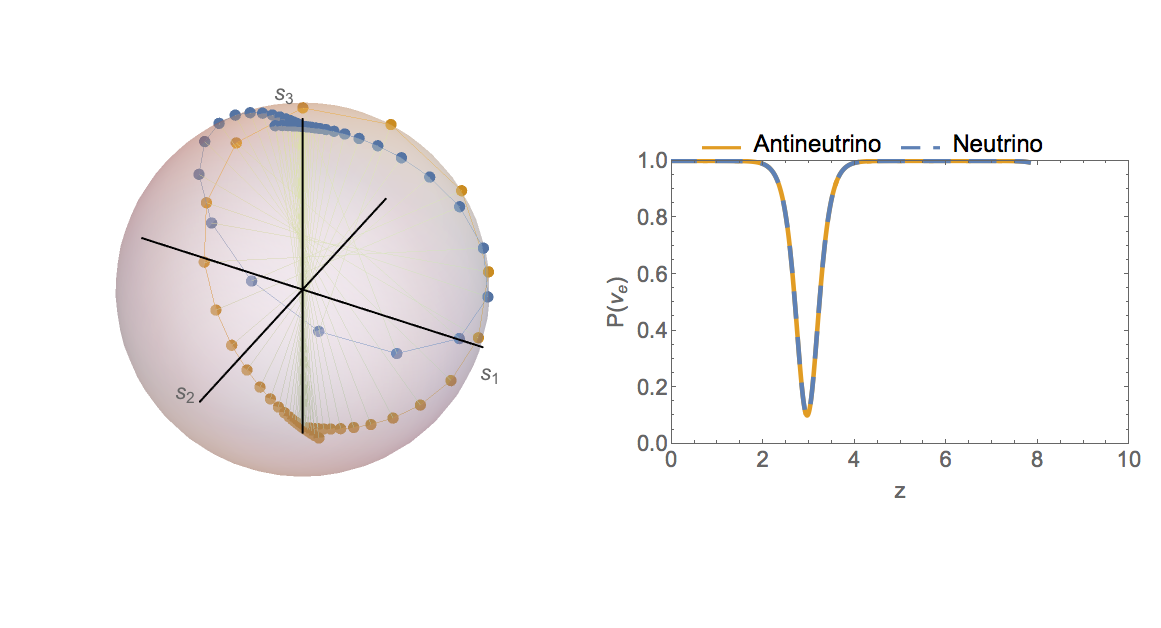
\includegraphics[width=\textwidth]{assets/bipolar-animation/bipolar-animie078.png}
   \end{figure}
   }
   \only<7>{
   \begin{figure}
      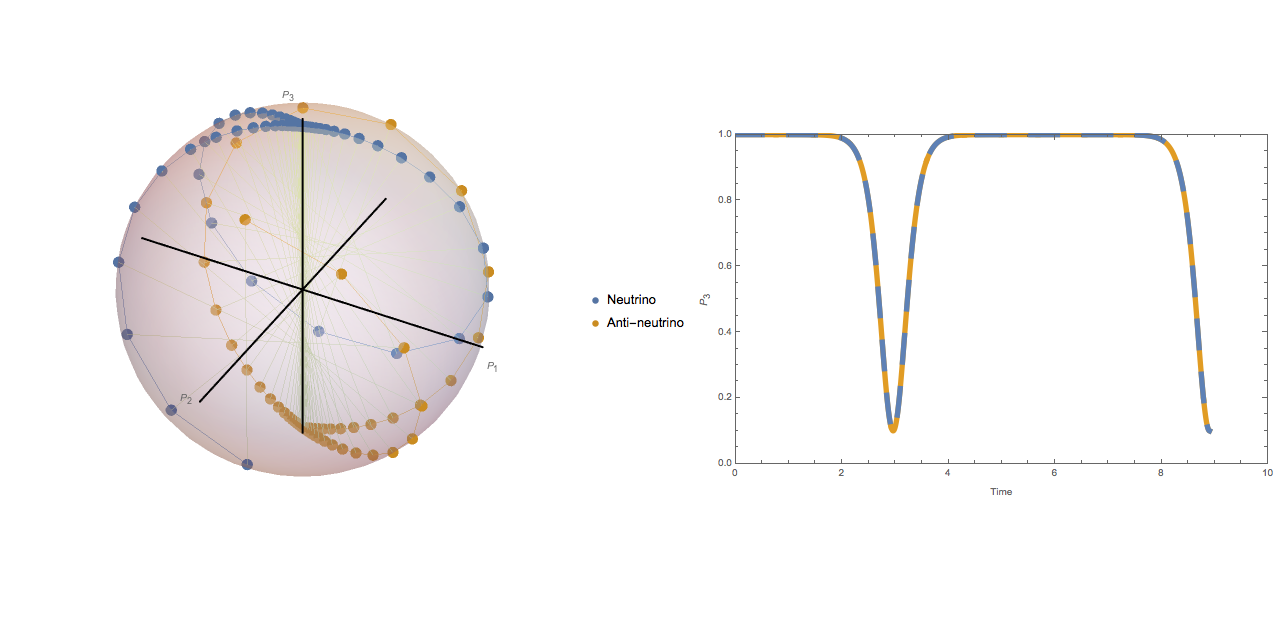
\includegraphics[width=\textwidth]{assets/bipolar-animation/bipolar-animie089.png}
   \end{figure}
   }
   \only<8>{
   \begin{figure}
      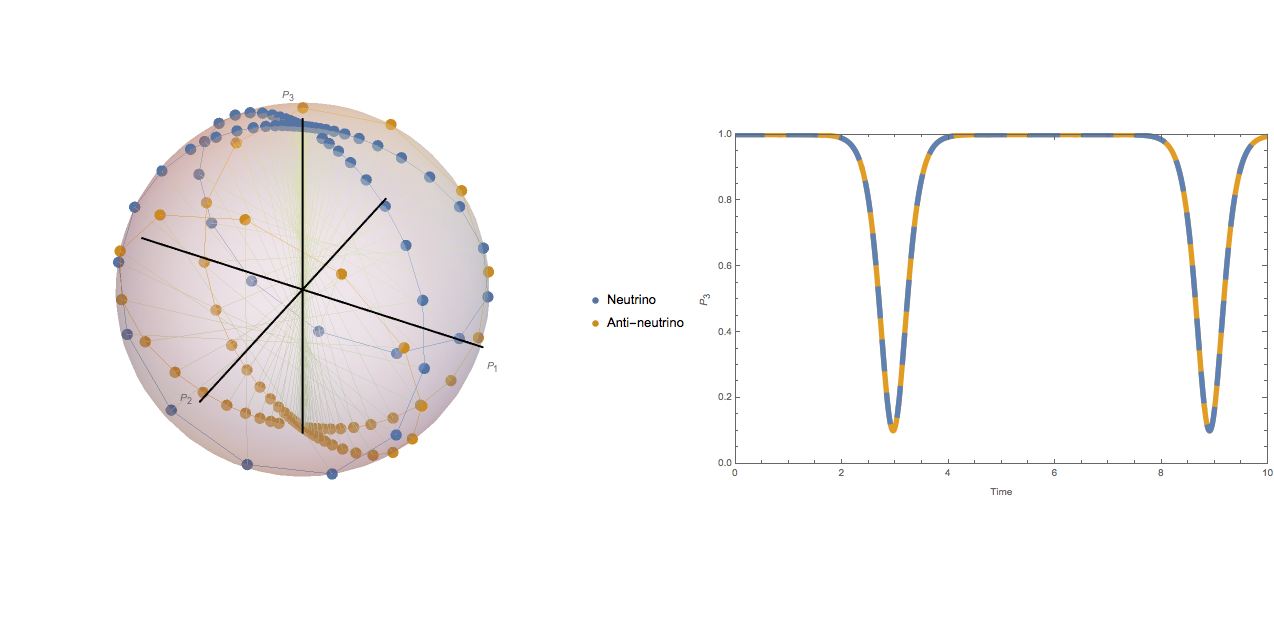
\includegraphics[width=\textwidth]{assets/bipolar-animation/bipolar-animie100.png}
   \end{figure}
   }
% \end{tcolorbox}

% \movie[autostart]{Movie}{assets/bipolar-movie.mp4}



\end{frame}






\subsection{Linear Stability Analysis}

\begin{frame}{Linear Stability Analysis}

   % \begin{textblock*}{100pt}(220pt,10pt)
   % \small
   % \begin{align*}
   %    H_{\nu\nu} = \frac{1}{2}\left( \mu_1 \rho_1 - \mu_2 \rho_2 \right)
   % \end{align*}
   % \end{textblock*}
   \vspace{-1em}
   \begin{figure}
      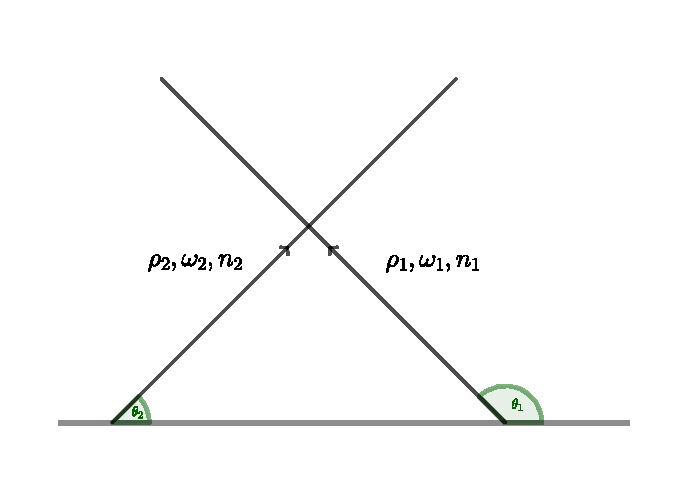
\includegraphics[width=\textwidth]{assets/two-beams-model-sym}
      \vspace{-2em}
      \caption*{$\rho_1$: neutrinos; $\rho_2$: antineutrinos}
   \end{figure}

\begin{columns}[T]
   \begin{column}{0.45\textwidth}

   \begin{equation*}
   \theta_1 =  5\pi/6, \theta_2 = \pi/6
   \end{equation*}
   \begin{align*}
      H_{\nu\nu} = \frac{1}{2}\left( \mu \rho_1 - \mu \rho_2 \right)
   \end{align*}
   \begin{equation*}
   i \partial_z \rho_i = \left[ H_i, \rho_i \right]
   \end{equation*}


   \end{column}%
\begin{column}{0.55\textwidth}
\pause
  \vspace{-1em}
   \begin{align*}
      \rho_i = \frac{1}{2}\begin{pmatrix}
      1 & \epsilon_i\\
      \epsilon_i^* & -1
      \end{pmatrix}
   \end{align*}
\pause
\begin{equation*}
i\partial_{z}\begin{pmatrix}
\epsilon_1 \\
\epsilon_2
\end{pmatrix} = \begin{pmatrix}
\mu/2 + \omega_{\mathrm v}   &  -\mu/2  \\
\mu/2 & -\omega_{\mathrm v} - \mu/2
\end{pmatrix}\begin{pmatrix}
\epsilon_1 \\
\epsilon_2
\end{pmatrix}
\end{equation*}


\end{column}%
\end{columns}



\end{frame}


\begin{frame}{Linear Stability Analysis}


Collective mode
\begin{equation*}
   \begin{pmatrix}
      \epsilon_1(z)\\
      \epsilon_2(z)
   \end{pmatrix} = \begin{pmatrix}
      \epsilon_1(0)\\
      \epsilon_2(0)
   \end{pmatrix} e^{i K_z z}
\end{equation*}


Eigenvalues or collective oscillation frequencies

\begin{equation*}
   K_z = \pm \sqrt{ \omega_{\mathrm v} ( \omega_{\mathrm v}+ \mu ) }
\end{equation*}

Identify the condition for complex eigenvalues

\begin{equation*}
   \omega_{\mathrm v} ( \omega_{\mathrm v}+ \mu ) < 0
\end{equation*}

\pause

\begin{itemize}
   \item Normal hierarchy: $\omega_{\mathrm v}>0$, requires $\cancel{ \mu  < -\omega_{\mathrm v} <0}$, no instability;
   \item Inverted hierarchy: $\omega_{\mathrm v}<0$, requires $\mu >\lvert \omega_{\mathrm v}\rvert$.
\end{itemize}

\pause

\begin{tcolorbox}
    \center
    $K_z$ is instability in $z$ direction for our model.
\end{tcolorbox}

\pause

\begin{tcolorbox}
    \centering
    Similar analysis can be done for all four dimensions $t, x, y, z$,
    \begin{equation*}
        \left( \Omega, K_x, K_y, K_z \right)
    \end{equation*}

 \end{tcolorbox}
\end{frame}



% \begin{frame}{Dispersion Relation}

%     \begin{tcolorbox}
%         \centering
%         Continuous emission angles?
%      \end{tcolorbox}

% \end{frame}

\subsection{Dispersion Relations}


\begin{frame}{ Dispersion Relation }

    \begin{tcolorbox}[standard jigsaw,opacityback=0]
        \color{white}
        Izaguirre, I., Raffelt, G., \& Tamborra, I. (2017). \emph{Fast Pairwise Conversion of Supernova Neutrinos: A Dispersion Relation Approach}. Physical Review Letters, 118(2), 021101.
    \end{tcolorbox}

    % \pause

    \begin{itemize}[<+->]
        \item Linear stability analysis $\rightarrow$ dispersion relation for $\Omega$ and $\mathbf K$.
        \item Instabilities and dispersion relation gaps are possibly related.
    \end{itemize}

    \end{frame}


\begin{frame}{Dispersion Relations}

Equation of motion for off-diagonal element of density matrix (Izaguirre et al, 2017)

\only<1>{
\begin{equation*}
   i(\partial_t + {\boldsymbol v} \cdot \boldsymbol{\nabla}_{\boldsymbol{r}} ) \epsilon (\boldsymbol v) =  v^\mu \left( \Lambda + \Phi \right)_\mu - \int d\Gamma' v^\mu v'_\mu G(\boldsymbol v') \epsilon(\boldsymbol v')
\end{equation*}
}


\only<2->{
\begin{equation*}
   i(\partial_t + {\boldsymbol v} \cdot \mathbf{\nabla}_{\boldsymbol{r}}  ) \epsilon (\boldsymbol v) = \colorbox{blue!50}{$ v^\mu$} ( \colorbox{red!50}{$\Lambda$} + \colorbox{ao!60}{$\Phi$} )_\mu - \int d\Gamma' v^\mu v'_\mu \colorbox{armygreen!70}{$G(\boldsymbol v')$} \epsilon(\boldsymbol v')
\end{equation*}
}


\pause

\begin{itemize}
    \item \colorbox{blue!50}{$ v^\mu$}:  four-velocity of neutrinos $(1, \boldsymbol v) $
    \item \colorbox{red!50}{$\Lambda$}: matter contribution $( \sqrt{2}G_{\mathrm F} n_{\mathrm e}, \sqrt{2}G_F n_e \boldsymbol v_{\mathrm e} )$
    \item \colorbox{ao!60}{$\Phi$}: neutrino flux $( \sqrt{2}G_{\mathrm F} n_{\nu}, \sqrt{2}G_F n_\nu \boldsymbol v )$
    \item \colorbox{armygreen!70}{$G(\boldsymbol{v}')$}: electron lepton number $\sqrt{2}G_{\mathrm F} \int_0^\infty \frac{E^2 dE}{2\pi^2} \left( n_{\nu_{\mathrm e}} - n_{\bar\nu_{\mathrm e}} \right)$
\end{itemize}



\end{frame}

\begin{frame}{Dispersion Relations}

\begin{tcolorbox}[standard jigsaw, opacityback=0]
    \color{white}
    Collective mode of off-diagonal element
\begin{equation*}
    \epsilon \to \tilde \epsilon e^{-i(\Omega t - \boldsymbol{ K}\cdot \boldsymbol{r} )}
\end{equation*}
\end{tcolorbox}

\pause

Replacement:
\begin{itemize}
    \item $\epsilon \to \tilde \epsilon$
    \item $\partial_t \to -i\Omega$, $\nabla_{\boldsymbol{r}}\to i \boldsymbol{K}$
\end{itemize}

\pause

\begin{tcolorbox}[standard jigsaw, opacityback=0]
    \color{white}
Collective mode

\only<3>{
\begin{equation*}
    v^\mu (K_\mu -( \Lambda + \Phi )_\mu ) \tilde\epsilon (\boldsymbol{v} ) = - \int d\Gamma' v^\mu v'_\mu G(\boldsymbol{v}') \tilde \epsilon (\boldsymbol{v}')
\end{equation*}
with $K_\mu \to ( \Omega, \boldsymbol{K} )$
}

\only<4>{
\begin{equation*}
    v^\mu \colorbox{red!50}{$\left( K_\mu -( \Lambda + \Phi )_\mu \right)$} \tilde\epsilon (\boldsymbol{v} ) = - \int d\Gamma' v^\mu v'_\mu G(\boldsymbol{v}') \tilde \epsilon (\boldsymbol{v}')
\end{equation*}
with $K_\mu \to ( \Omega, \boldsymbol{K} )$
}

\only<5->{
\begin{equation*}
    v^\mu \colorbox{red!50}{$k_\mu$} \tilde\epsilon (\boldsymbol{v} ) = - \int d\Gamma' v^\mu v'_\mu G(\boldsymbol{v}') \tilde \epsilon (\boldsymbol{v}')
\end{equation*}
with \colorbox{red!50}{$k_\mu \to ( \omega, \boldsymbol{k} )$}
}



\end{tcolorbox}

\only<6>{
Without neutrino self-interaction: $v^\mu k_\mu = 0$
}

\end{frame}

\begin{frame}{Dispersion Relations}

\only<3>{
\begin{textblock*}{80pt}(200pt,5pt)

    % \begin{tcolorbox}[standard jigsaw, opacityback=0]
        \begin{equation*}
            \color{white}
            v^\mu k_\mu \tilde\epsilon (\boldsymbol{v} ) = - \int d\Gamma' v^\mu v'_\mu G(\boldsymbol{v}') \tilde \epsilon (\boldsymbol{v}')
        \end{equation*}
    % \end{tcolorbox}
\end{textblock*}
}

% \begin{tcolorbox}[standard jigsaw, opacityback=0]
%     \color{white}
% \begin{equation*}
%     v^\mu K_\mu \tilde\epsilon (\boldsymbol{v} ) = \cancel{- \int d\Gamma' v^\mu v'_\mu G(\boldsymbol{v}') \tilde \epsilon (\boldsymbol{v}') } = 0
% \end{equation*}
% \end{tcolorbox}

Rewrite
\begin{align*}
    &- \int d\Gamma' \colorbox{red!50}{$v^\mu$} v'_\mu G(\boldsymbol{v}') \tilde \epsilon (\boldsymbol{v}') \\
    =& \colorbox{red!50}{$v^\mu$} \colorbox{blue!50}{$\left(- \int d\Gamma'  v'_\mu G(\boldsymbol{v}') \tilde \epsilon (\boldsymbol{v}') \right)$} \\
    \equiv&   \colorbox{red!50}{$v^\mu$} \colorbox{blue!50}{$a_\mu$}
\end{align*}

\pause

EoM


\begin{equation*}
    v^\mu k_\mu \tilde \epsilon (\boldsymbol{v}) = v^\mu a_\mu
\end{equation*}
\pause
{\centering
$\Longrightarrow$
\begin{equation*}
    \tilde \epsilon (\boldsymbol{v}) = v^\mu a_\mu/v^\mu k_\mu
\end{equation*}
}
Collect all terms of $a_\mu$

\begin{equation*}
    v^\mu \left( \delta_\mu^\nu +  \int d\Gamma' \frac{ G(\boldsymbol{ v}') v'_\mu v^\nu }{ v^\alpha k_\alpha }   \right) a_\nu = 0
\end{equation*}

\end{frame}


\begin{frame}{Dispersion Relations}

% \begin{textblock*}{100pt}(250pt,5pt)
% \begin{equation*}
%     \tilde \epsilon (\boldsymbol{v}) = v^\mu a_\mu/v^\mu K_\mu
% \end{equation*}
% \end{textblock*}

\begin{tcolorbox}[standard jigsaw, opacityback=0, coltext=white]
    % \color{white}
Axially symmetric: $v^\alpha k_\alpha = \omega (1 - n \cos \theta)$ where $n = \lvert \boldsymbol{k} \rvert / \omega $
\end{tcolorbox}

\begin{columns}[T]
    \begin{column}{0.5\textwidth}
Condition for nontrivial solutions of $a_\mu$,
\only<1>{
\begin{equation*}
    v^\mu \left( \omega \delta^\nu_{\phantom{\nu}\mu} + N^\nu_{\phantom{\nu}\mu} \right) a_\nu =0
\end{equation*}
}
\only<2->{
\begin{equation*}
    v^\mu \colorbox{blue!50}{$\left( \omega \delta^\nu_{\phantom{\nu}\mu} + N^\nu_{\phantom{\nu}\mu} \right) a_\nu$} =0
\end{equation*}
}

\only<3->{
    \centering
    $\Rightarrow$
    \begin{equation*}
    \left( \omega \delta^\nu_{\phantom{\nu}\mu} + N^\nu_{\phantom{\nu}\mu} \right) a_\nu =0
    \end{equation*}
}

\only<4->{
    \centering
    $\Rightarrow$
\begin{equation*}
   \operatorname{Det}\left(\omega I + N \right) = 0,
\end{equation*}
}


\end{column}

\begin{column}{0.5\textwidth}




   \begin{equation*}
      I_n(\theta)=\int_{\cos\theta_2}^{\cos\theta_1} d\cos\theta G(\theta) \frac{\cos^n\theta}{1 - n \cos\theta }
   \end{equation*}




   \begin{equation*}
      N^\mu_{\phantom{\mu}\nu} \to
   \end{equation*}
\begin{equation*}
    \small
  \begin{pmatrix}
   \frac{1}{2}  I_0 & 0 & 0 & -\frac{1}{2}I_1\\
   0 & -\frac{1}{4}(I_0-I_2) & 0 & 0\\
   0 & 0 & -\frac{1}{4}(I_0-I_2) & 0 \\
   \frac{1}{2}I_1 & 0 & 0 & -\frac{1}{2}I_2
   \end{pmatrix}
   \end{equation*}





\end{column}

\end{columns}

% \only<5->{
%
%    \begin{tcolorbox}
%     \vspace{-0.8em}
%    \begin{equation*}
%    \omega = \frac{1}{4}(I_0-I_2), \quad -\frac{1}{4}\left(I_0-I_2\pm \sqrt{ (I_0-2I_1+I_2)(I_0+2I_1+I_2) }\right)
%    \end{equation*}
%    \end{tcolorbox}
% }

\end{frame}


\begin{frame}{Dispersion Relations}

   \begin{textblock*}{100pt}(230pt,5pt)
      \begin{equation*}
           a_\mu = -\int d\Gamma' v'_{\mu} G(\boldsymbol{v}') \tilde \epsilon (\boldsymbol{v}')
      \end{equation*}
   \end{textblock*}

   \begin{equation*}
       \omega =
               {\colorbox{red!50}{$\frac{1}{4}(I_0-I_2)$}}
               , \qquad
               \colorbox{blue!50}{$-\frac{1}{4}\left(I_0-I_2\pm \sqrt{ (I_0-2I_1+I_2)(I_0+2I_1+I_2) }\right)$}
   \end{equation*}




   \begin{itemize}
       \item \colorbox{red!50}{MAA solution}: Related to flavor evolution due to multiple azimuthal angles
       \item \colorbox{blue!50}{MZA solution}: Related to flavor evolution due to multiple zenith angles
   \end{itemize}

   % \tikzstyle{na} = [baseline=-.5ex]






   % \begin{equation*}
   %     \omega =
   %     \tikz[baseline]{
   %             \node[fill=red!50,anchor=base] (t1)
   %             {\colorbox{red!50}{$\frac{1}{4}(I_0-I_2)$}}
   %             }
   %             , \qquad
   %             \tikz[baseline]{
   %             \node[fill=blue!50, anchor=base] (t2)
   %             {
   %             \colorbox{blue!50}{$-\frac{1}{4}\left(I_0-I_2\pm \sqrt{ (I_0-2I_1+I_2)(I_0+2I_1+I_2) }\right)$}
   %             };
   %         }
   % \end{equation*}
   %
   %
   %
   %
   % \begin{itemize}
   %     \item \colorbox{blue!50}{MAA solution}
   %         \tikz[na]\node [coordinate] (n2) {};
   %         : Related to axial symmetry breaking
   %     \item \colorbox{red!50}{MZA solution}: Related to azimuthal symmetry breaking
   %         \tikz[na]\node [coordinate] (n3) {};
   % \end{itemize}







   % Now it's time to draw some edges between the global nodes. Note that we
   % have to apply the 'overlay' style.
   % \begin{tikzpicture}[overlay]
   %         \path[->]<1-> (n2) edge [bend right] (t1);
   %         \path[->]<1-> (n3) edge [bend right=20] (t2);
   % \end{tikzpicture}







\end{frame}

\begin{frame}{Dispersion Relations and Instabilities}


    \begin{textblock*}{100pt}(230pt,10pt)
      % \begin{tcolorbox}
         Modified version of Fig. 1 in Izaguirre et al, 2017;
      % \end{tcolorbox}
    \end{textblock*}

    \begin{figure}
        % \begin{tcolorbox}
            % \color{white}
        % \centering
        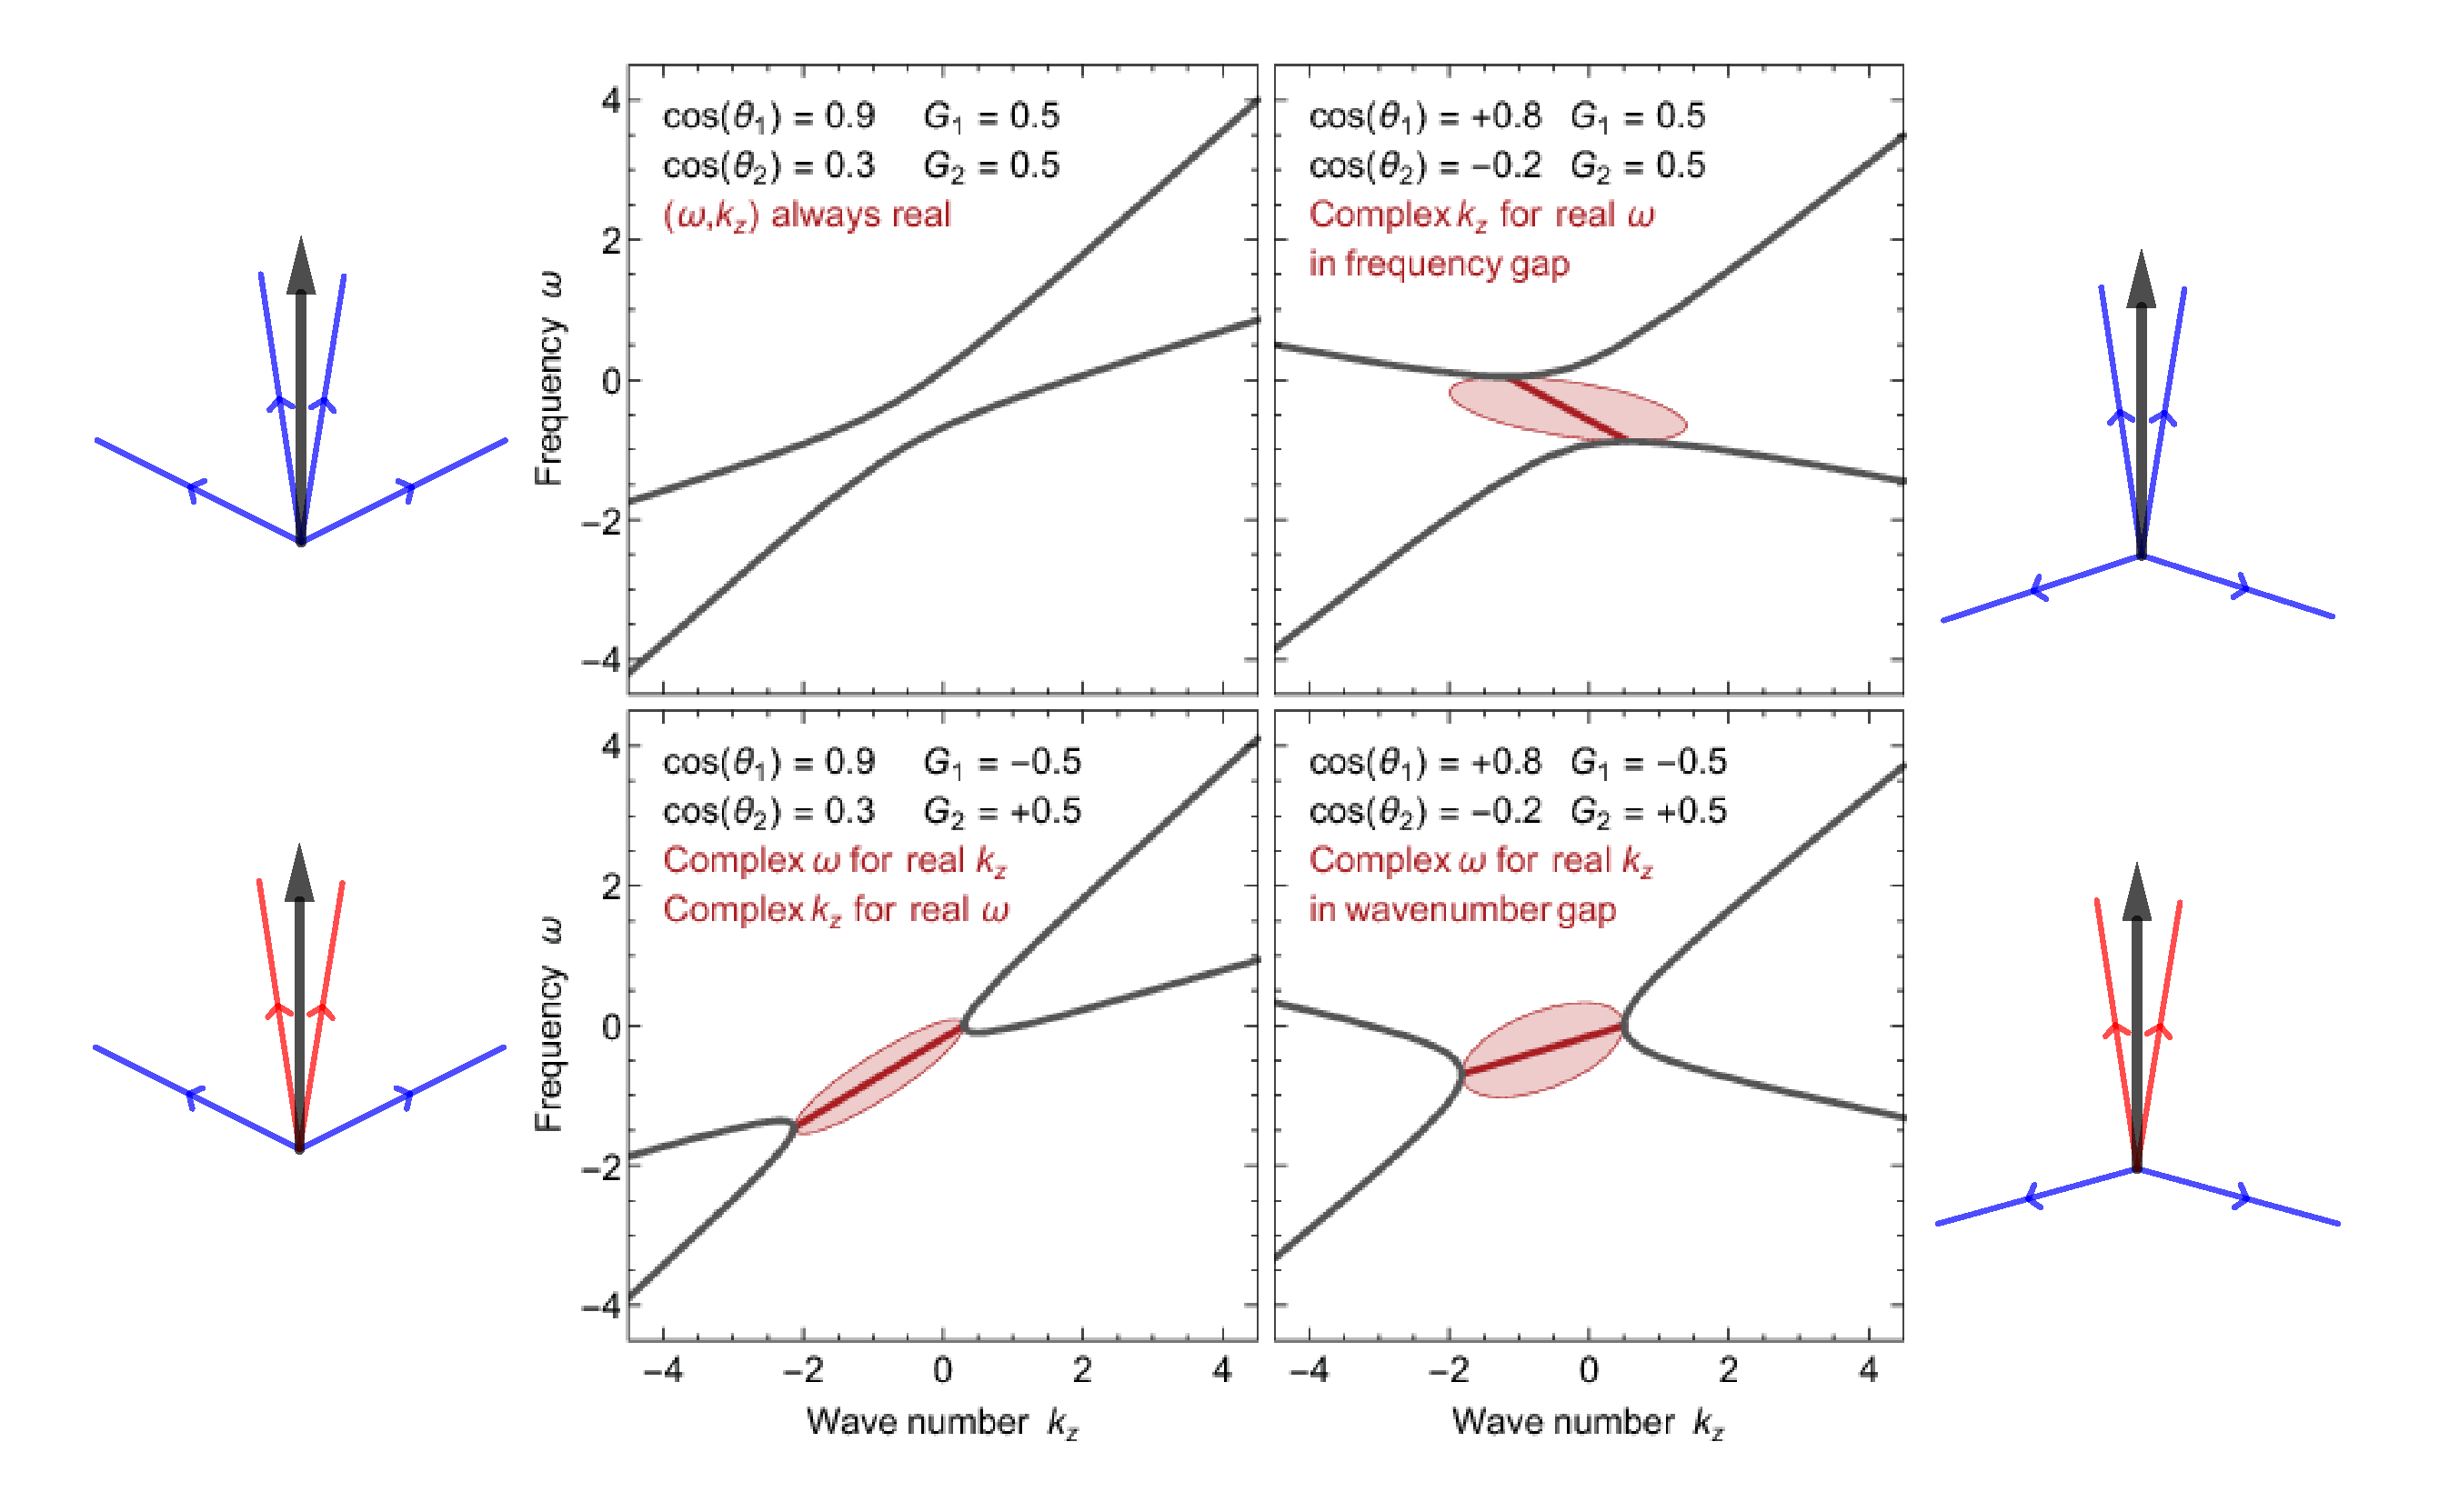
\includegraphics[width=\textwidth]{assets/dr/two-zenith-angles-with-configuration}
        % \end{tcolorbox}
        \caption*{Two zenith angles}
    \end{figure}


% \begin{figure}
%     \begin{tcolorbox}
%         \color{white}
%     \centering
%     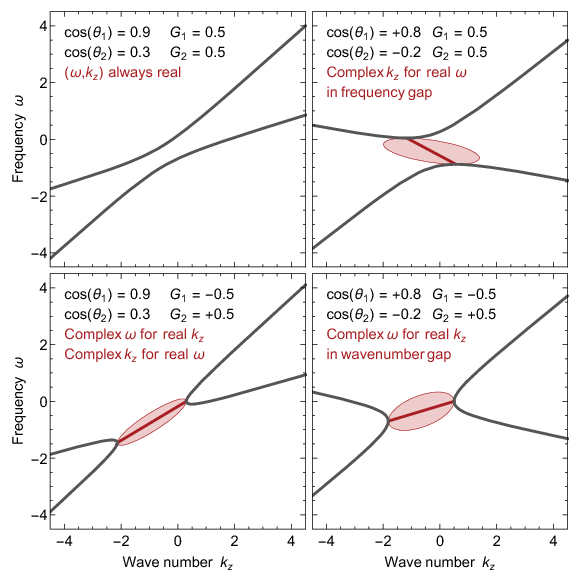
\includegraphics[width=0.8\textwidth]{assets/dr/dr-two-beams.png}
%     \end{tcolorbox}
%
% \end{figure}

%    \begin{columns}[T]

% \begin{column}{0.5\textwidth}
%    \begin{figure}
%      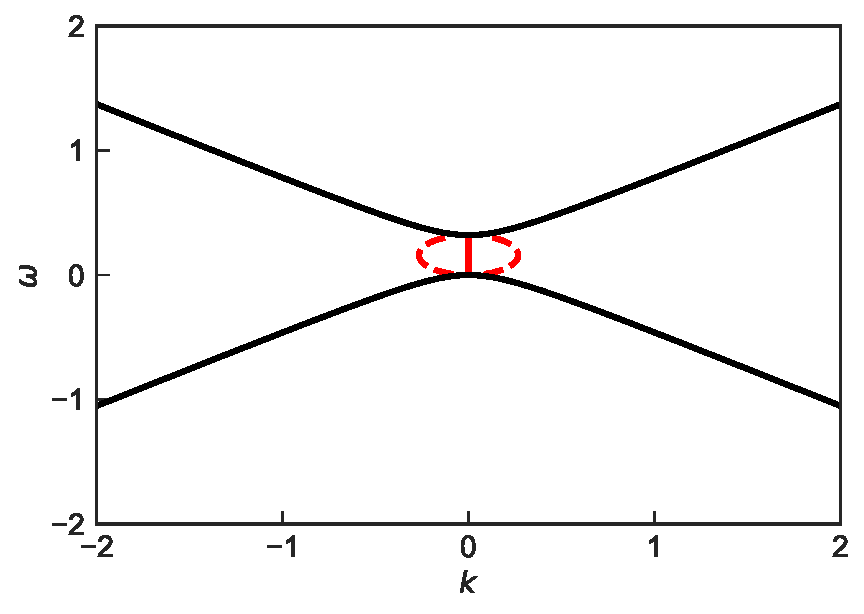
\includegraphics[width=\linewidth]{assets/dr/spectDBWC1DRDBMAAPltBlob.pdf}
%      \caption*{MAA solutions}
%   \end{figure}
% \end{column}

% \begin{column}{0.5\textwidth}
%    \begin{figure}
%       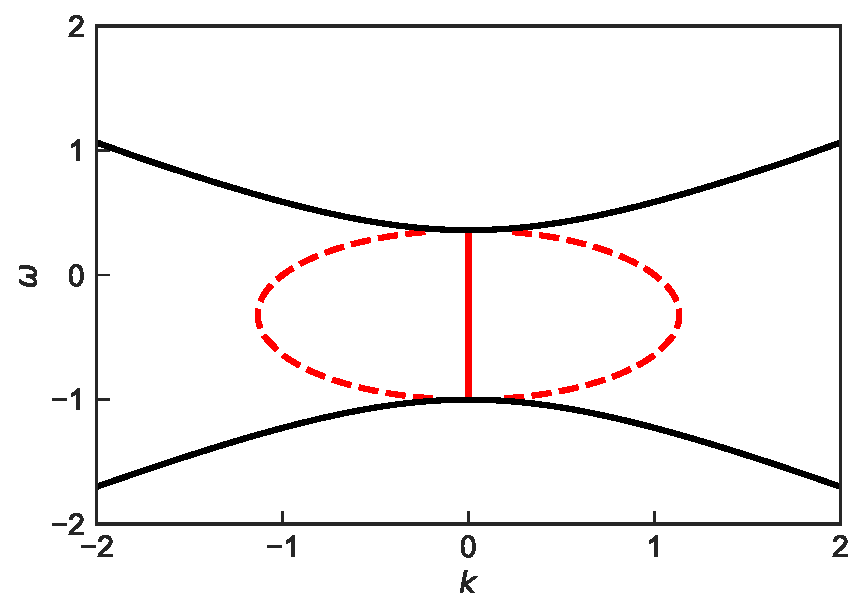
\includegraphics[width=\linewidth]{assets/dr/spectDBWC1DRDBMZAPltBlob.pdf}
%       \caption*{ MZA solutions}
%    \end{figure}
% \end{column}

%    \end{columns}

% \begin{tcolorbox}
%    \centering
%    Two zenith angles
% \end{tcolorbox}

\end{frame}

\begin{frame}{Dispersion Relations and Instabilities}

   \begin{tcolorbox}[standard jigsaw,opacityback=0]
      \color{white}
      \small
      Izaguirre, I., Raffelt, G., \& Tamborra, I. (2017). \emph{Fast Pairwise Conversion of Supernova Neutrinos: A Dispersion Relation Approach}. Physical Review Letters, 118(2), 021101.
   \end{tcolorbox}
\vspace{-0.7em}
   \begin{tcolorbox}
% \begin{figure}
%    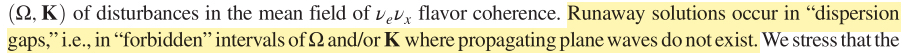
\includegraphics[width=\textwidth]{assets/dr/izaguirre1.jpg}
% \end{figure}

\begin{columns}[T]
   \begin{column}{0.5\textwidth}
      \begin{figure}
         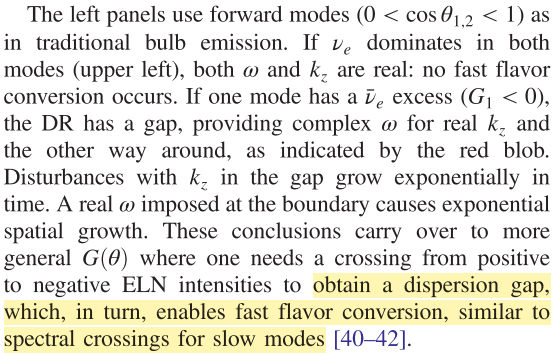
\includegraphics[width=\textwidth]{assets/dr/izaguirre2.jpg}
      \end{figure}
   \end{column}%
   \begin{column}{0.5\textwidth}
      \begin{figure}
         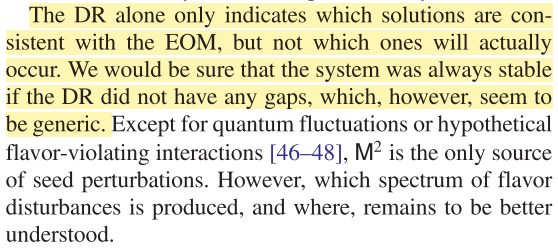
\includegraphics[width=\textwidth]{assets/dr/izaguirre3.jpg}
      \end{figure}
   \end{column}
\end{columns}
\end{tcolorbox}


\vspace{-0.8em}
\begin{enumerate}
   % \item Instabilities occur in gaps.
   \item Gaps lead to Instabilities.
   \item Instabilities do not occur without gap.
\end{enumerate}

\end{frame}



\begin{frame}{Dispersion Relations and Instabilities}

\centering
      Three zenith angles

   \begin{columns}[T]

\begin{column}{0.5\textwidth}
   \begin{figure}
     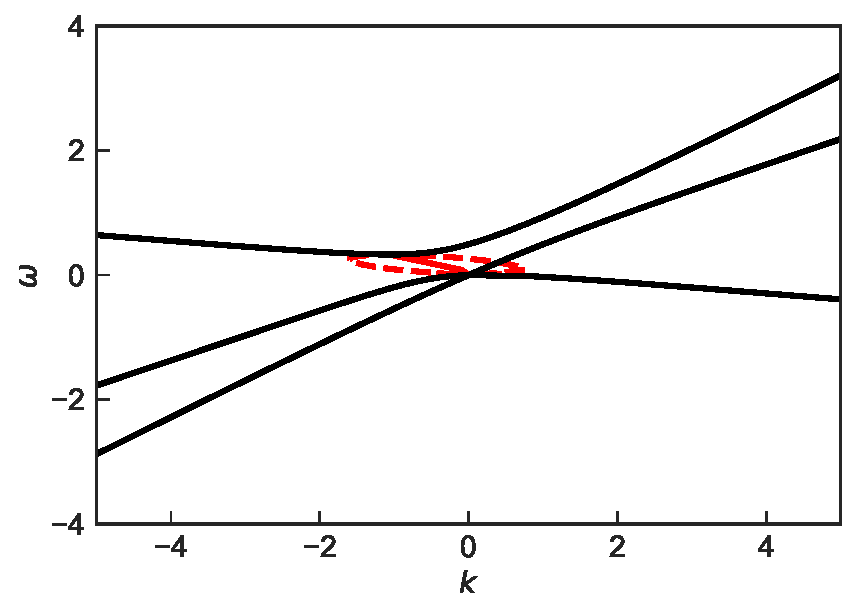
\includegraphics[width=\linewidth]{assets/dr/spectDB3WC4DRDBMAAPltBlob.pdf}
     \caption*{MAA solutions}
  \end{figure}
\end{column}

\begin{column}{0.5\textwidth}
   \begin{figure}
      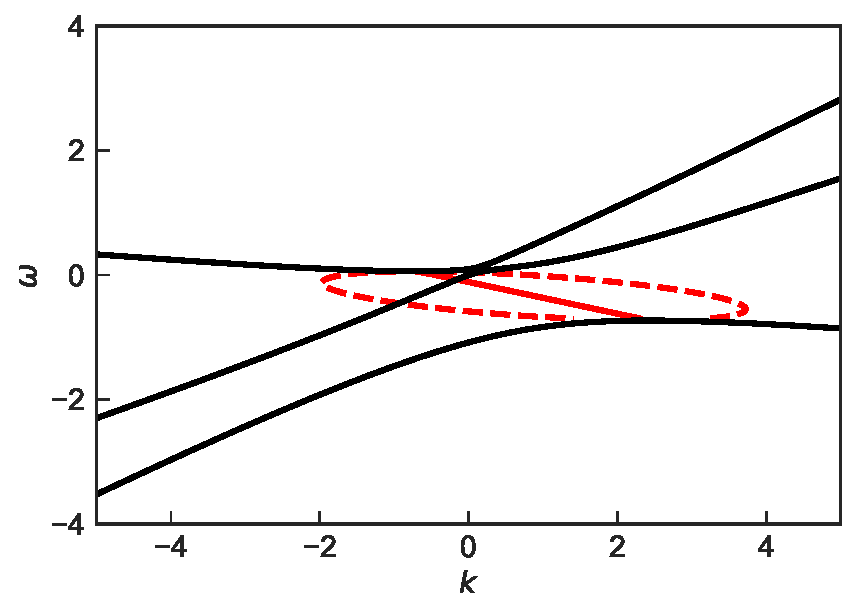
\includegraphics[width=\linewidth]{assets/dr/spectDB3WC4DRDBMZAPltBlob.pdf}
      \caption*{ MZA solutions}
   \end{figure}
\end{column}

   \end{columns}



\pause
\begin{tcolorbox}[halign=center]
   Cubic equation of $k=\lvert \boldsymbol{k} \rvert$ $\Rightarrow$ 3 solutions of $k$ for given $\omega$
\end{tcolorbox}



\pause
   \begin{tcolorbox}
      \centering
      % \begin{itemize}
         % \item
         \color{black}Instabilities occur without gaps.
      % \end{itemize}
   \end{tcolorbox}



\end{frame}


\begin{frame}{Dispersion Relations and Instabilities}



   \begin{figure}
      \minipage{0.49\textwidth}
      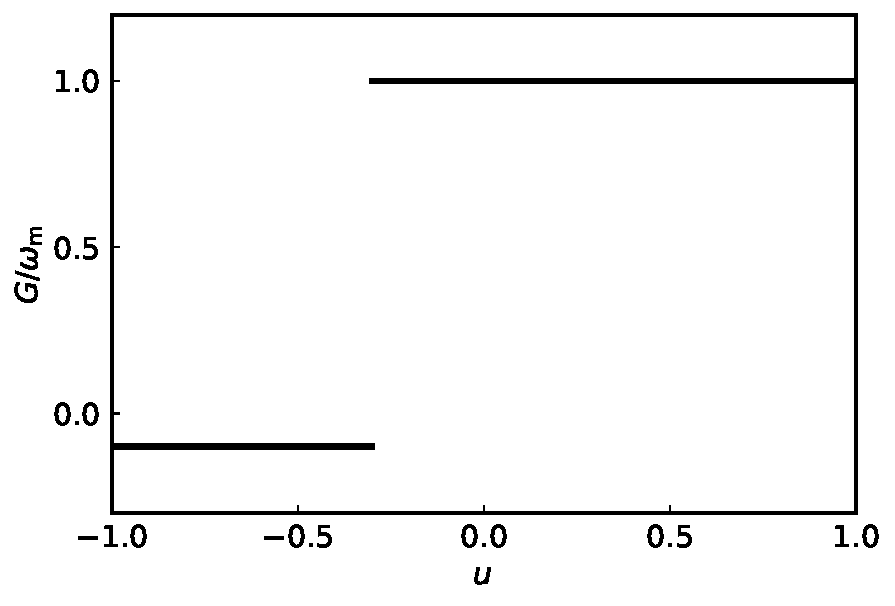
\includegraphics[width=\linewidth]{assets/dr/boxSpectPlt}
      \caption*{Box spectrum: $-0.1$ for $u\in [-1,-0.3)$; $1$ for $u\in [-0.3,1]$}
      \endminipage\hfill
      \minipage{0.49\textwidth}
      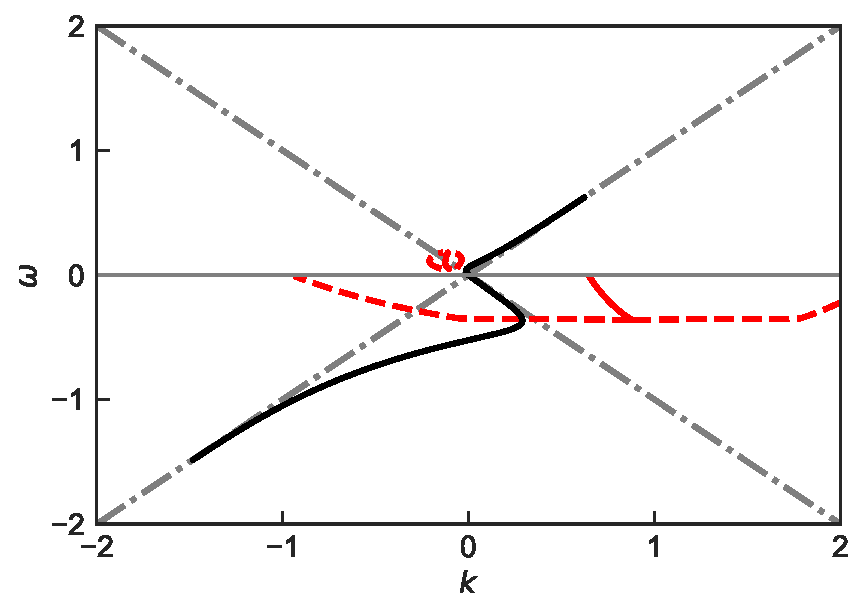
\includegraphics[width=\linewidth]{assets/dr/spectBoxC1MZADRPltBlob.pdf}
      \caption*{MZA solution: no gaps yet unstable in some regions}
      \endminipage\hfill
    %   \caption*{Dispersion relation and linear stability analysis for box spectrum. The box spectrum is defined to be $-0.1$ within range $u\in [-1,-0.3)$ and $1$ within range $u\in [-0.3,1]$. Left panel shows the dispersion relation and the complex $k$ for real $\omega$ for MAA solution. Right panel is the corresponding result for MZA solution. Dash-dotted gray lines are $\omega= \pm k$ which sets the boundaries of the forbidden region for dispersion relation.
    %    }
    \pause
    \begin{tcolorbox}
      \centering
      Instabilities occur without gaps.
    \end{tcolorbox}
   \end{figure}



\end{frame}



\begin{frame}{Dispersion Relations and Instabilities}


       \begin{textblock*}{100pt}(230pt,10pt)
           Remake of Fig.3 of Izaguirre et al, 2017
       \end{textblock*}

Define $u=\cos\theta$

Garching spectrum:

   \begin{figure}
      \minipage{0.49\textwidth}
        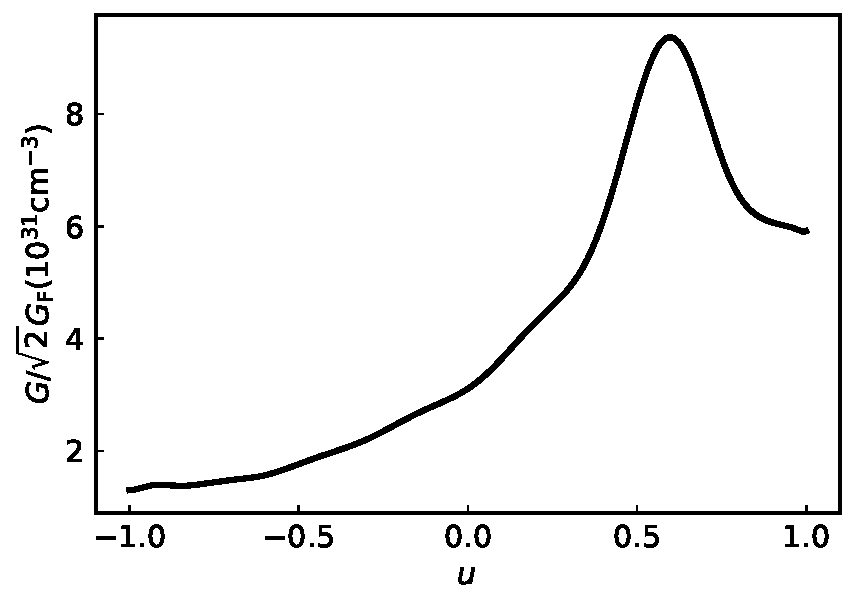
\includegraphics[width=\linewidth]{assets/dr/spectGarchingPlt.pdf}
        \caption*{Garching spectrum $G(u)$}
      \endminipage\hfill
      \minipage{0.49\textwidth}
      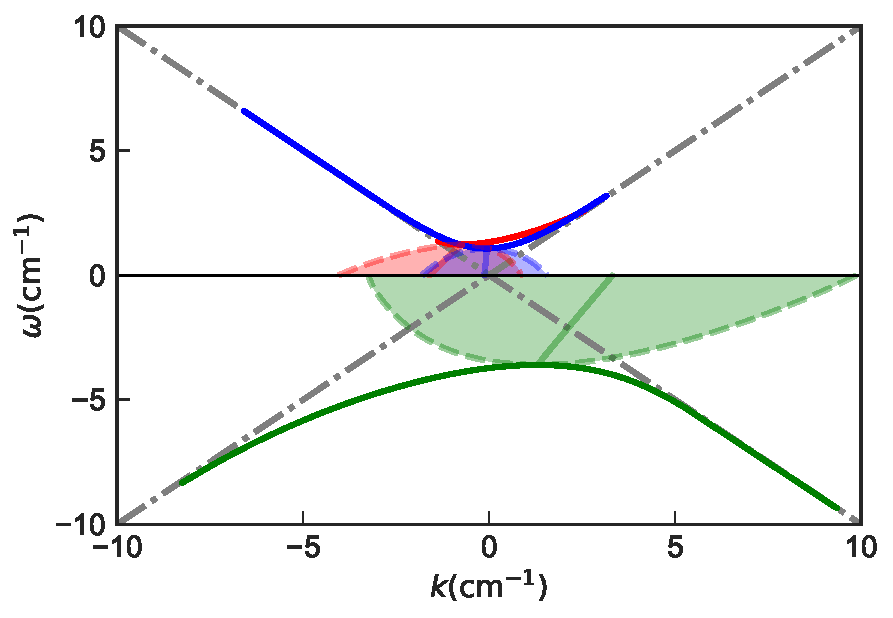
\includegraphics[width=\linewidth]{assets/dr/spectGarchingDRLSAPltBlob.pdf}
      \caption*{ MAA: red; MZA: blue and green }
      \endminipage\hfill
    %   \caption*{Dispersion relation and linear stability analysis (right panel) for a spectrum constructed from Garching 1D simulation data (left panel). Solid red line is dispersion relation for MAA solution while blue and green lines are for MZA solutions. Light red (blue and green) blob is instability for MAA (MZA) solution.
    %    }
   \end{figure}

\pause
\begin{tcolorbox}
   \begin{itemize}
      \item
      \color{black}MAA solutions: unstable region stops at $\omega\to 0$
      \item
      \color{black} MZA solutions: instabilities are different for region $\omega>0$ and $\omega<0$.
   \end{itemize}
\end{tcolorbox}
\pause
\begin{tcolorbox}
   \color{black} Instabilities might occur in gaps of DR and $\omega=0$ if there is any.
\end{tcolorbox}

\end{frame}








\subsection{Summary of Collective Oscillations}

\begin{frame}{Summary of Dispersion Relations}

\begin{itemize}
   \item Neutrino oscillation instabilities might occur in DR gaps.
   \item Neutrino oscillation instabilities might occur even if DR has no gaps.
   \item If there exists gaps, gaps should be defined as the gap between dispersion relation and $\omega=0$ instead of the gaps between dispersion relation curves.
\end{itemize}

\end{frame}
